\documentclass{beamer}
\usetheme{Copenhagen}
\usepackage{flexiprogram}
\usepackage{wrapfig}
\usepackage[usenames,dvipsnames]{pstricks}
\usepackage{epsfig}
\usepackage{pst-func}
\usepackage{pst-grad} % For gradients
\usepackage{pst-plot} % For axes
\usepackage{pst-node}
\usepackage{url}
%\usepackage{enumerate}

% \usepackage[labelfont={bf}]{caption}

\bibliographystyle{plain}

\title{Android Based Greenhouse Monitoring (And Harvesting) Using Accurate And Automated Bot Guidance System}
\author{Devendra Bhave (114050004) \\ \and Mohd Vasimuddin (114050007) \\ \and Meenakshi Verma (123050014) \\ \and Mukund Lahoti (123050018)}
\date{\today}

\setbeamertemplate{footline}[frame number]

\begin{document}

\frame{\titlepage}

\frame{\frametitle{Contents}\tableofcontents} 

\section{Introduction}

\frame{\frametitle{Wish List}
 \begin{itemize}
  \item Automated greenhouse monitoring
  \item Automated harvesting
 \end{itemize}
} 

\frame{\frametitle{Requirements}
  \begin{itemize}
   \item Bot guidance system
   \item Battery charging facility
   \item Right tools
  \end{itemize}
}

\section{System Design}

\frame{\frametitle{Environment Description}
% Generated with LaTeXDraw 2.0.8
% Fri Sep 28 11:04:02 IST 2012
% \usepackage[usenames,dvipsnames]{pstricks}
% \usepackage{epsfig}
% \usepackage{pst-grad} % For gradients
% \usepackage{pst-plot} % For axes
\scalebox{0.75} % Change this value to rescale the drawing.
{
\begin{pspicture}(0,-3.325)(15.197187,3.365)
\psframe[linewidth=0.04,dimen=outer](7.1771874,-0.925)(3.5771875,-3.125)
\psframe[linewidth=0.04,dimen=outer](9.177188,0.075)(5.5771875,-2.125)
\psarc[linewidth=0.04](7.3771877,0.075){1.8}{0.0}{180.0}
\psarc[linewidth=0.04](5.3771877,-0.925){1.8}{0.0}{180.0}
\psline[linewidth=0.04cm](7.1771874,-3.125)(9.177188,-2.125)
\psline[linewidth=0.04cm](7.1771874,-0.925)(9.177188,0.075)
\psline[linewidth=0.04cm](4.5771875,0.675)(6.5771875,1.675)
\psline[linewidth=0.04cm](3.5771875,-3.125)(5.5771875,-2.125)
\psline[linewidth=0.04cm](3.5771875,-0.925)(5.5771875,0.075)
\psline[linewidth=0.04cm](5.3771877,-2.525)(6.1771874,-2.525)
\psline[linewidth=0.04cm](5.3771877,-2.525)(5.3771877,-2.925)
\psline[linewidth=0.04cm](6.1771874,-2.525)(6.1771874,-2.925)
\psline[linewidth=0.04cm](5.3771877,-2.925)(6.1771874,-2.925)
\psline[linewidth=0.04cm](5.3771877,-2.525)(5.7771873,-2.325)
\psline[linewidth=0.04cm](5.7771873,-2.325)(6.5771875,-2.325)
\psline[linewidth=0.04cm](6.5771875,-2.325)(6.1771874,-2.525)
\psline[linewidth=0.04cm](6.5771875,-2.325)(6.5771875,-2.725)
\psline[linewidth=0.04cm](6.1771874,-2.925)(6.5771875,-2.725)
\usefont{T1}{ptm}{m}{n}
\rput(5.225625,1.78){Greenhouse}
\psframe[linewidth=0.04,dimen=outer](7.5771875,2.075)(7.1771874,1.875)
\psframe[linewidth=0.04,dimen=outer](1.9971875,-0.125)(0.1971875,-1.125)
\psframe[linewidth=0.04,dimen=outer](3.1771874,3.075)(2.3771875,-3.325)
\psframe[linewidth=0.04,dimen=outer](13.177188,-0.925)(9.577188,-3.125)
\psframe[linewidth=0.04,dimen=outer](15.177188,0.075)(11.577188,-2.125)
\psarc[linewidth=0.04](13.377188,0.075){1.8}{0.0}{180.0}
\psarc[linewidth=0.04](11.377188,-0.925){1.8}{0.0}{180.0}
\psline[linewidth=0.04cm](13.177188,-3.125)(15.177188,-2.125)
\psline[linewidth=0.04cm](13.177188,-0.925)(15.177188,0.075)
\psline[linewidth=0.04cm](10.577188,0.675)(12.577188,1.675)
\psline[linewidth=0.04cm](9.577188,-3.125)(11.577188,-2.125)
\psline[linewidth=0.04cm](9.577188,-0.925)(11.577188,0.075)
\psline[linewidth=0.04cm](11.377188,-2.525)(12.177188,-2.525)
\psline[linewidth=0.04cm](11.377188,-2.525)(11.377188,-2.925)
\psline[linewidth=0.04cm](12.177188,-2.525)(12.177188,-2.925)
\psline[linewidth=0.04cm](11.377188,-2.925)(12.177188,-2.925)
\psline[linewidth=0.04cm](11.377188,-2.525)(11.777187,-2.325)
\psline[linewidth=0.04cm](11.777187,-2.325)(12.577188,-2.325)
\psline[linewidth=0.04cm](12.577188,-2.325)(12.177188,-2.525)
\psline[linewidth=0.04cm](12.577188,-2.325)(12.577188,-2.725)
\psline[linewidth=0.04cm](12.177188,-2.925)(12.577188,-2.725)
\usefont{T1}{ptm}{m}{n}
\rput(11.225625,1.78){Greenhouse}
\psframe[linewidth=0.04,dimen=outer](13.577188,2.075)(13.177188,1.875)
\psline[linewidth=0.04cm](7.3771877,2.075)(7.3771877,2.475)
\psline[linewidth=0.04cm](13.377188,2.075)(13.377188,2.475)
\psline[linewidth=0.04cm](3.1771874,2.475)(13.377188,2.475)
\psarc[linewidth=0.04](7.3771877,1.975){0.2}{225.0}{-45.0}
\psarc[linewidth=0.04](7.3771877,1.975){0.3}{225.0}{-45.0}
\psarc[linewidth=0.04](7.3771877,1.975){0.4}{225.0}{-45.0}
\psarc[linewidth=0.04](13.377188,1.975){0.2}{225.0}{-45.0}
\psarc[linewidth=0.04](13.377188,1.975){0.3}{225.0}{-45.0}
\psarc[linewidth=0.04](13.377188,1.975){0.4}{225.0}{-45.0}
\rput{-211.16742}(10.514545,-7.5239124){\psarc[linewidth=0.04](6.3064766,-2.2957106){0.2}{225.0}{-45.0}}
\rput{-211.16742}(10.514545,-7.5239124){\psarc[linewidth=0.04](6.3064766,-2.2957106){0.3}{225.0}{-45.0}}
\rput{-211.16742}(10.514545,-7.5239124){\psarc[linewidth=0.04](6.3064766,-2.2957106){0.4}{225.0}{-45.0}}
\rput{-211.16742}(21.648499,-10.629155){\psarc[linewidth=0.04](12.306477,-2.2957106){0.2}{225.0}{-45.0}}
\rput{-211.16742}(21.648499,-10.629155){\psarc[linewidth=0.04](12.306477,-2.2957106){0.3}{225.0}{-45.0}}
\rput{-211.16742}(21.648499,-10.629155){\psarc[linewidth=0.04](12.306477,-2.2957106){0.4}{225.0}{-45.0}}
\rput{-211.16742}(2.886594,-0.5964881){\psarc[linewidth=0.04](1.5264769,0.10428932){0.2}{225.0}{-45.0}}
\rput{-211.16742}(2.886594,-0.5964881){\psarc[linewidth=0.04](1.5264769,0.10428932){0.3}{225.0}{-45.0}}
\rput{-211.16742}(2.886594,-0.5964881){\psarc[linewidth=0.04](1.5264769,0.10428932){0.4}{225.0}{-45.0}}
\usefont{T1}{ptm}{m}{n}
\rput(1.080625,-1.42){Android Phone}
\usefont{T1}{ptm}{m}{n}
\rput(2.7482812,2.1){I}
\usefont{T1}{ptm}{m}{n}
\rput(2.7853124,1.540759){n}
\usefont{T1}{ptm}{m}{n}
\rput(2.7457812,0.8602679){t}
\usefont{T1}{ptm}{m}{n}
\rput(2.7653124,0.2763393){e}
\usefont{T1}{ptm}{m}{n}
\rput(2.7571876,-0.35540178){r}
\usefont{T1}{ptm}{m}{n}
\rput(2.7853124,-0.98745537){n}
\usefont{T1}{ptm}{m}{n}
\rput(2.7653124,-1.6198214){e}
\usefont{T1}{ptm}{m}{n}
\rput(2.7457812,-2.3){t}
\usefont{T1}{ptm}{m}{n}
\rput(10.368594,3.18){WiFi Access Points}
\psline[linewidth=0.04cm,arrowsize=0.05291667cm 2.0,arrowlength=1.4,arrowinset=0.4]{<-}(7.5771875,2.075)(10.377188,2.875)
\psline[linewidth=0.04cm,arrowsize=0.05291667cm 2.0,arrowlength=1.4,arrowinset=0.4]{->}(10.377188,2.875)(13.177188,2.075)
\end{pspicture} 
}

WiFi has speed and range advantage over ZigBee and Bluetooth.
}

\frame{\frametitle{Bot Description}
% Generated with LaTeXDraw 2.0.8
% Fri Sep 28 11:06:57 IST 2012
% \usepackage[usenames,dvipsnames]{pstricks}
% \usepackage{epsfig}
% \usepackage{pst-grad} % For gradients
% \usepackage{pst-plot} % For axes
\scalebox{0.7} % Change this value to rescale the drawing.
{
\begin{pspicture}(0,-4.92)(15.8,4.9)
\psframe[linewidth=0.04,dimen=outer](3.6,-0.3)(0.0,-2.5)
\psframe[linewidth=0.04,dimen=outer](5.6,0.7)(2.0,-1.5)
\psarc[linewidth=0.04](3.8,0.7){1.8}{0.0}{180.0}
\psarc[linewidth=0.04](1.8,-0.3){1.8}{0.0}{180.0}
\psline[linewidth=0.04cm](3.6,-2.5)(5.6,-1.5)
\psline[linewidth=0.04cm](3.6,-0.3)(5.6,0.7)
\psline[linewidth=0.04cm](1.0,1.3)(3.0,2.3)
\psline[linewidth=0.04cm](0.0,-2.5)(2.0,-1.5)
\psline[linewidth=0.04cm](0.0,-0.3)(2.0,0.7)
\psline[linewidth=0.04cm](1.8,-1.9)(2.6,-1.9)
\psline[linewidth=0.04cm](1.8,-1.9)(1.8,-2.3)
\psline[linewidth=0.04cm](2.6,-1.9)(2.6,-2.3)
\psline[linewidth=0.04cm](1.8,-2.3)(2.6,-2.3)
\psline[linewidth=0.04cm](1.8,-1.9)(2.2,-1.7)
\psline[linewidth=0.04cm](2.2,-1.7)(3.0,-1.7)
\psline[linewidth=0.04cm](3.0,-1.7)(2.6,-1.9)
\psline[linewidth=0.04cm](3.0,-1.7)(3.0,-2.1)
\psline[linewidth=0.04cm](2.6,-2.3)(3.0,-2.1)
\pscircle[linewidth=0.04,linestyle=dashed,dash=0.16cm 0.16cm,dimen=outer](2.4,-2.1){0.8}
\psline[linewidth=0.04cm](7.0,-0.9)(7.6,-0.3)
\psline[linewidth=0.04cm](11.6,-0.3)(11.0,-0.9)
\psline[linewidth=0.04cm](11.6,-0.3)(11.6,-2.1)
\psline[linewidth=0.04cm](11.6,-2.1)(11.0,-2.7)
\pscircle[linewidth=0.04,dimen=outer](9.1,-2.6){1.1}
\psline[linewidth=0.04cm](10.2,-2.7)(11.0,-2.7)
\psline[linewidth=0.04cm](11.0,-2.7)(11.0,-0.9)
\psline[linewidth=0.04cm](11.0,-0.9)(7.0,-0.9)
\psline[linewidth=0.04cm](7.0,-0.9)(7.0,-2.7)
\psline[linewidth=0.04cm](7.0,-2.7)(8.0,-2.7)
\psarc[linewidth=0.04](9.9,-2.0){1.1}{-80.0}{-40.0}
\psline[linewidth=0.04cm](8.2,1.5)(8.2,-0.9)
\psline[linewidth=0.04cm](8.2,1.5)(8.8,2.1)
\psline[linewidth=0.04cm](8.8,2.1)(8.8,-0.3)
\psline[linewidth=0.04cm](8.8,-0.3)(8.2,-0.9)
\psline[linewidth=0.04cm](8.2,1.5)(7.8,1.5)
\psline[linewidth=0.04cm](7.8,1.5)(7.8,-0.9)
\psline[linewidth=0.04cm](7.8,1.5)(8.4,2.1)
\psline[linewidth=0.04cm](8.4,2.1)(8.8,2.1)
\psline[linewidth=0.04cm](7.6,-0.3)(7.8,-0.3)
\psline[linewidth=0.04cm](9.8,-0.1)(9.8,-0.7)
\psline[linewidth=0.04cm](9.8,-0.1)(10.4,-0.1)
\psline[linewidth=0.04cm](10.4,-0.1)(10.4,-0.7)
\psline[linewidth=0.04cm](9.8,-0.7)(10.4,-0.7)
\psline[linewidth=0.04cm](9.8,-0.1)(11.4,2.1)
\pscircle[linewidth=0.04,dimen=outer](11.6,2.1){0.2}
\psline[linewidth=0.04cm](11.6,1.9)(10.4,-0.1)
\psline[linewidth=0.04cm](11.6,2.3)(14.1,2.9)
\psline[linewidth=0.04cm](11.6,1.9)(14.1,2.7)
\pscircle[linewidth=0.04,dimen=outer](14.1,2.8){0.3}
\pscircle[linewidth=0.04,dimen=outer](14.1,2.8){0.1}
\psline[linewidth=0.04cm](10.6,-0.1)(10.6,-0.5)
\psline[linewidth=0.04cm](10.6,-0.5)(10.4,-0.7)
\psline[linewidth=0.04cm](10.6,0.1)(10.6,-0.1)
\psline[linewidth=0.04cm](10.6,0.1)(10.4,-0.1)
\psline[linewidth=0.04cm](11.6,1.9)(10.6,0.1)
\psline[linewidth=0.04cm](11.6,-0.3)(10.6,-0.3)
\psline[linewidth=0.04cm](9.8,-0.3)(8.8,-0.3)
\psellipse[linewidth=0.04,dimen=outer](8.5,1.3)(0.1,0.2)
\psline[linewidth=0.04cm](14.2,3.1)(14.4,3.3)
\psline[linewidth=0.04cm](14.4,3.3)(14.4,2.9)
\psline[linewidth=0.04cm](14.4,2.9)(14.6,2.9)
\psline[linewidth=0.04cm](14.6,2.9)(14.4,2.7)
\psline[linewidth=0.04cm](14.4,2.7)(14.6,2.5)
\psline[linewidth=0.04cm](14.6,2.5)(14.2,2.5)
\psline[linewidth=0.04cm](14.2,2.5)(14.2,2.3)
\psline[linewidth=0.04cm](14.2,2.3)(14.0,2.5)
\psline[linewidth=0.04cm](14.0,2.5)(13.8,2.3)
\psline[linewidth=0.04cm](13.8,2.3)(13.8,2.5)
\psline[linewidth=0.04cm](13.8,2.5)(13.8,2.7)
\psline[linewidth=0.04cm](13.8,2.7)(13.6,2.7)
\psline[linewidth=0.04cm](13.6,2.7)(13.8,2.9)
\psline[linewidth=0.04cm](13.8,2.9)(13.6,3.1)
\psline[linewidth=0.04cm](13.6,3.1)(14.0,3.1)
\psline[linewidth=0.04cm](14.0,3.1)(14.0,3.3)
\psline[linewidth=0.04cm](14.0,3.3)(14.2,3.1)
\pscircle[linewidth=0.04,linestyle=dashed,dash=0.16cm 0.16cm,dimen=outer](10.9,0.0){4.9}
\psline[linewidth=0.04cm,linestyle=dashed,dash=0.16cm 0.16cm](2.2,-1.3)(8.2,4.1)
\psline[linewidth=0.04cm,linestyle=dashed,dash=0.16cm 0.16cm](2.2,-2.9)(10.2,-4.9)
\usefont{T1}{ptm}{m}{n}
\rput(8.483438,2.405){Android Phone}
\usefont{T1}{ptm}{m}{n}
\rput(9.697344,-1.195){FireBird Bot}
\usefont{T1}{ptm}{m}{n}
\rput(1.6484375,2.405){Greenhouse}
\usefont{T1}{ptm}{m}{n}
\rput(11.126094,3.805){Robotic Arm}
\usefont{T1}{ptm}{m}{n}
\rput(14.121718,0.205){Circular Saw}
\psline[linewidth=0.04cm,arrowsize=0.05291667cm 2.0,arrowlength=1.4,arrowinset=0.4]{->}(11.0,3.5)(11.0,1.3)
\psline[linewidth=0.04cm,arrowsize=0.05291667cm 2.0,arrowlength=1.4,arrowinset=0.4]{<-}(14.4,2.5)(14.4,0.5)
\end{pspicture} 
}

}

\frame{\frametitle{Bot Guidance System}
 Location Error: Difference between physical location of the Bot in \alert{real world} and location known 
 to Bot guidance system
 \vspace{\baselineskip}
 \pause

 Desired properties of the Bot guidance system:
 \begin{enumerate}
  \item Accurate: Fixed known bound on Bot location error
  \item Automated: No human intervention needed for Bot navigation
 \end{enumerate}
 \vspace{\baselineskip}
 \pause
 
 Our design is both \alert{accurate} and \alert{automated}.
}

\frame{\frametitle{Bot Guidance System}
 Guidance System knows precise location of the Bot.
 \pause
 \vspace{\baselineskip}
 
 Design offers \alert{mathematical guarantee} that location error will \alert{never} exceed 
 constant bound $\delta_{max}$ no matter how long you use it.
}

\frame{\frametitle{Relevant Terminologies}
 \structure{Accuracy}: the degree of closeness of measurements of a quantity to that quantity's actual (true) value \cite{wikiap}
 
 \vspace{\baselineskip}
 \structure{Precision}: the degree to which repeated measurements under unchanged conditions show the same results \cite{wikiap}

 \vspace{\baselineskip}
% Generated with LaTeXDraw 2.0.8
% Fri Sep 28 13:30:35 IST 2012
% \usepackage[usenames,dvipsnames]{pstricks}
% \usepackage{epsfig}
% \usepackage{pst-grad} % For gradients
% \usepackage{pst-plot} % For axes
\scalebox{1} % Change this value to rescale the drawing.
{
\begin{pspicture}(0,-1.4925)(8.72,1.4525)
\definecolor{color65}{rgb}{0.9411764705882353,0.0,0.0}
\pscircle[linewidth=0.04,dimen=outer](1.0,0.4525){0.4}
\pscircle[linewidth=0.04,dimen=outer](1.0,0.4525){0.6}
\pscircle[linewidth=0.04,dimen=outer](1.0,0.4525){0.8}
\pscircle[linewidth=0.04,dimen=outer](1.0,0.4525){1.0}
\pscircle[linewidth=0.04,dimen=outer](3.6,0.4525){0.4}
\pscircle[linewidth=0.04,dimen=outer](3.6,0.4525){0.6}
\pscircle[linewidth=0.04,dimen=outer](3.6,0.4525){0.8}
\pscircle[linewidth=0.04,dimen=outer](3.6,0.4525){1.0}
\psdots[dotsize=0.12,linecolor=color65](0.5,0.5525)
\psdots[dotsize=0.12,linecolor=color65](1.1,0.7525)
\psdots[dotsize=0.12,linecolor=color65](1.3,0.1525)
\psdots[dotsize=0.12,linecolor=color65](0.9,0.1525)
\psdots[dotsize=0.12,linecolor=color65](2.96,1.0325)
\psdots[dotsize=0.12,linecolor=color65](2.92,0.8525)
\psdots[dotsize=0.12,linecolor=color65](3.08,0.8725)
\psdots[dotsize=0.12,linecolor=color65](3.18,1.0125)
\usefont{T1}{ptm}{m}{n}
\rput(1.0628124,-0.8425){High accuracy,}
\usefont{T1}{ptm}{m}{n}
\rput(3.6153126,-0.8025){Low accuracy}
\usefont{T1}{ptm}{m}{n}
\rput(1.015625,-1.2425){Low precision}
\usefont{T1}{ptm}{m}{n}
\rput(3.6260939,-1.2025){High precision}
\psline[linewidth=0.04cm,arrowsize=0.05291667cm 2.0,arrowlength=1.4,arrowinset=0.4]{<-}(5.5,0.7525)(5.5,-0.6475)
\psline[linewidth=0.04cm,arrowsize=0.05291667cm 2.0,arrowlength=1.4,arrowinset=0.4]{->}(5.5,-0.6475)(8.7,-0.6475)
\psline[linewidth=0.04cm](6.1,0.5525)(6.1,-0.6475)
\psline[linewidth=0.04cm,linestyle=dashed,dash=0.16cm 0.16cm](7.3,0.5525)(7.3,-0.6475)
\psline[linewidth=0.04cm,arrowsize=0.05291667cm 2.0,arrowlength=1.4,arrowinset=0.4]{<->}(6.1,0.9525)(7.3,0.9525)
\usefont{T1}{ptm}{m}{n}
\rput(6.7775,1.2575){Accuracy}
\psline[linewidth=0.04cm,arrowsize=0.05291667cm 2.0,arrowlength=1.4,arrowinset=0.4]{<->}(6.7,-1.0475)(7.9,-1.0475)
\usefont{T1}{ptm}{m}{n}
\rput(7.35625,-1.3425){Precision}
\rput(7.3,-0.7375){\psGauss[sigma=0.30, linecolor=red, linewidth=0.04cm]{-0.6}{0.6}}
\end{pspicture} 
}

}

\frame{\frametitle{Characterizing Location Error}
 Sources of location error:
 \begin{itemize}
  \item Quantization error in wheel counter
  \item Missed wheel counts
  \item Wheel circumference measurement error
  \item Slight differences in wheel diameters
 \end{itemize}
 
 \vspace{\baselineskip}
 Small errors \alert{accumulate} over time to catastrophic level.
 \vspace{\baselineskip}
 \begin{columns}
 \begin{column}{0.4\textwidth}
 $
 \begin{array}{l}
  \textrm{Location error, E} \\
  = f(\textrm{distance travelled}) \\
  = \kappa \cdot d
 \end{array}
 $
 
 \end{column}

 \begin{column}{0.4\textwidth}  
 % Generated with LaTeXDraw 2.0.8
  % Thu Sep 27 19:22:26 IST 2012
  % \usepackage[usenames,dvipsnames]{pstricks}
  % \usepackage{epsfig}
  % \usepackage{pst-grad} % For gradients
  % \usepackage{pst-plot} % For axes
  \scalebox{1} % Change this value to rescale the drawing.
  {
  \begin{pspicture}(0,-1.3325)(2.6828125,1.3325)
  \psline[linewidth=0.04cm,arrowsize=0.05291667cm 2.0,arrowlength=1.4,arrowinset=0.4]{<-}(0.4628125,1.1125)(0.4628125,-0.6875)
  \psline[linewidth=0.04cm,arrowsize=0.05291667cm 2.0,arrowlength=1.4,arrowinset=0.4]{->}(0.4628125,-0.6875)(2.6628125,-0.6875)
  \psline[linewidth=0.04cm](0.4628125,-0.4875)(2.2628126,0.3125)
  \usefont{T1}{ptm}{m}{n}
  \rput(1.2745312,-1.1825){Distance}
  \usefont{T1}{ptm}{m}{n}
  \rput{-270.0}(0.3625,0.1075){\rput(0.1203125,0.2175){Location Error}}
  \end{pspicture} 
  }
 \end{column}
 \end{columns}
}

\frame{\frametitle{Design of Bot Guidance System}
% Generated with LaTeXDraw 2.0.8
% Thu Sep 27 22:57:43 IST 2012
% \usepackage[usenames,dvipsnames]{pstricks}
% \usepackage{epsfig}
% \usepackage{pst-grad} % For gradients
% \usepackage{pst-plot} % For axes
\scalebox{1} % Change this value to rescale the drawing.
{
\begin{pspicture}(0,-3.2)(10.0,3.2)
\definecolor{color476b}{rgb}{0.0,0.9215686274509803,0.0}
\psframe[linewidth=0.04,dimen=outer,fillstyle=solid,fillcolor=darkgray](10.0,3.2)(0.0,-3.2)
\psframe[linewidth=0.04,dimen=outer,fillstyle=solid,fillcolor=color476b](3.0,2.2)(1.0,1.4)
\psframe[linewidth=0.04,linecolor=white,dimen=outer,fillstyle=solid](9.6,2.8)(0.4,2.6)
\psframe[linewidth=0.04,linecolor=white,dimen=outer,fillstyle=solid](0.6,2.8)(0.4,-2.8)
\psframe[linewidth=0.04,linecolor=white,dimen=outer,fillstyle=solid](3.6,2.8)(3.4,-2.8)
\psframe[linewidth=0.04,linecolor=white,dimen=outer,fillstyle=solid](6.6,2.8)(6.4,-2.8)
\psframe[linewidth=0.04,linecolor=white,dimen=outer,fillstyle=solid](9.6,2.8)(9.4,-2.8)
\psframe[linewidth=0.04,linecolor=white,dimen=outer,fillstyle=solid](9.6,1.0)(0.4,0.8)
\psframe[linewidth=0.04,linecolor=white,dimen=outer,fillstyle=solid](9.6,-0.8)(0.4,-1.0)
\psframe[linewidth=0.04,linecolor=white,dimen=outer,fillstyle=solid](9.6,-2.6)(0.4,-2.8)
\psframe[linewidth=0.04,dimen=outer,fillstyle=solid,fillcolor=color476b](6.0,2.2)(4.0,1.4)
\psframe[linewidth=0.04,dimen=outer,fillstyle=solid,fillcolor=color476b](9.0,2.2)(7.0,1.4)
\psframe[linewidth=0.04,dimen=outer,fillstyle=solid,fillcolor=color476b](3.0,0.4)(1.0,-0.4)
\psframe[linewidth=0.04,dimen=outer,fillstyle=solid,fillcolor=color476b](6.0,0.4)(4.0,-0.4)
\psframe[linewidth=0.04,dimen=outer,fillstyle=solid,fillcolor=color476b](9.0,0.4)(7.0,-0.4)
\psframe[linewidth=0.04,dimen=outer,fillstyle=solid,fillcolor=color476b](3.0,-1.4)(1.0,-2.2)
\psframe[linewidth=0.04,dimen=outer,fillstyle=solid,fillcolor=color476b](6.0,-1.4)(4.0,-2.2)
\psframe[linewidth=0.04,dimen=outer,fillstyle=solid,fillcolor=color476b](9.0,-1.4)(7.0,-2.2)
\end{pspicture} 
}
}

\frame{\frametitle{Design of Bot Guidance System}
% Generated with LaTeXDraw 2.0.8
% Thu Sep 27 22:58:47 IST 2012
% \usepackage[usenames,dvipsnames]{pstricks}
% \usepackage{epsfig}
% \usepackage{pst-grad} % For gradients
% \usepackage{pst-plot} % For axes
\scalebox{1} % Change this value to rescale the drawing.
{
\begin{pspicture}(0,-3.2)(10.0,3.2)
\definecolor{color476b}{rgb}{0.0,0.9215686274509803,0.0}
\definecolor{color22b}{rgb}{0.9411764705882353,0.0,0.0}
\psframe[linewidth=0.04,dimen=outer,fillstyle=solid,fillcolor=darkgray](10.0,3.2)(0.0,-3.2)
\psframe[linewidth=0.04,dimen=outer,fillstyle=solid,fillcolor=color476b](3.0,2.2)(1.0,1.4)
\psframe[linewidth=0.04,linecolor=white,dimen=outer,fillstyle=solid](9.6,2.8)(0.4,2.6)
\psframe[linewidth=0.04,linecolor=white,dimen=outer,fillstyle=solid](0.6,2.8)(0.4,-2.8)
\psframe[linewidth=0.04,linecolor=white,dimen=outer,fillstyle=solid](3.6,2.8)(3.4,-2.8)
\psframe[linewidth=0.04,linecolor=white,dimen=outer,fillstyle=solid](6.6,2.8)(6.4,-2.8)
\psframe[linewidth=0.04,linecolor=white,dimen=outer,fillstyle=solid](9.6,2.8)(9.4,-2.8)
\psframe[linewidth=0.04,linecolor=white,dimen=outer,fillstyle=solid](9.6,1.0)(0.4,0.8)
\psframe[linewidth=0.04,linecolor=white,dimen=outer,fillstyle=solid](9.6,-0.8)(0.4,-1.0)
\psframe[linewidth=0.04,linecolor=white,dimen=outer,fillstyle=solid](9.6,-2.6)(0.4,-2.8)
\psframe[linewidth=0.04,dimen=outer,fillstyle=solid,fillcolor=color476b](6.0,2.2)(4.0,1.4)
\psframe[linewidth=0.04,dimen=outer,fillstyle=solid,fillcolor=color476b](9.0,2.2)(7.0,1.4)
\psframe[linewidth=0.04,dimen=outer,fillstyle=solid,fillcolor=color476b](3.0,0.4)(1.0,-0.4)
\psframe[linewidth=0.04,dimen=outer,fillstyle=solid,fillcolor=color476b](6.0,0.4)(4.0,-0.4)
\psframe[linewidth=0.04,dimen=outer,fillstyle=solid,fillcolor=color476b](9.0,0.4)(7.0,-0.4)
\psframe[linewidth=0.04,dimen=outer,fillstyle=solid,fillcolor=color476b](3.0,-1.4)(1.0,-2.2)
\psframe[linewidth=0.04,dimen=outer,fillstyle=solid,fillcolor=color476b](6.0,-1.4)(4.0,-2.2)
\psframe[linewidth=0.04,dimen=outer,fillstyle=solid,fillcolor=color476b](9.0,-1.4)(7.0,-2.2)
\psframe[linewidth=0.04,linecolor=color22b,dimen=outer,fillstyle=solid,fillcolor=color22b](0.6,1.6)(0.4,1.4)
\psframe[linewidth=0.04,linecolor=color22b,dimen=outer,fillstyle=solid,fillcolor=color22b](3.0,2.8)(2.8,2.6)
\psframe[linewidth=0.04,linecolor=color22b,dimen=outer,fillstyle=solid,fillcolor=color22b](6.6,2.0)(6.4,1.8)
\psframe[linewidth=0.04,linecolor=color22b,dimen=outer,fillstyle=solid,fillcolor=color22b](4.2,1.0)(4.0,0.8)
\psframe[linewidth=0.04,linecolor=color22b,dimen=outer,fillstyle=solid,fillcolor=color22b](0.6,-1.4)(0.4,-1.6)
\psframe[linewidth=0.04,linecolor=color22b,dimen=outer,fillstyle=solid,fillcolor=color22b](3.6,-2.2)(3.4,-2.4)
\psframe[linewidth=0.04,linecolor=color22b,dimen=outer,fillstyle=solid,fillcolor=color22b](8.8,2.8)(8.6,2.6)
\psframe[linewidth=0.04,linecolor=color22b,dimen=outer,fillstyle=solid,fillcolor=color22b](7.2,-0.8)(7.0,-1.0)
\psframe[linewidth=0.04,linecolor=color22b,dimen=outer,fillstyle=solid,fillcolor=color22b](9.6,0.4)(9.4,0.2)
\psframe[linewidth=0.04,linecolor=color22b,dimen=outer,fillstyle=solid,fillcolor=color22b](7.4,-2.6)(7.2,-2.8)
\end{pspicture} 
}
}

\frame{\frametitle{Design of Bot Guidance System}
Design summary:
\begin{itemize}
 \item Map of arena is precisely known
 \item Use white line to follow path
 \item Add checkpoints to mitigate location errors
\end{itemize}

\vspace{\baselineskip}
\pause

Checkpoint: A co-ordinate on the map whose location is \alert{accurately} known.

\vspace{\baselineskip}
\pause

Bot senses checkpoint when it passes over it and updates its current location eliminating location error.
}

\frame{\frametitle{Source of Error in Detecting Checkpoint}
Checkpoint sensing is not perfect. It introduces small amount of location error $\epsilon$.

\vspace{\baselineskip}
This error is due to delay between instant when the Bot passes over checkpoint and the instant when
guidance system updates Bot location.

\vspace{\baselineskip}
If Bot is moving with speed 10 cm/sec and delay in updating its location is 20 msec, error $\epsilon$ is 2 mm.
}

\frame{\frametitle{Error Characteristics Of Bot Guidance System}
% Generated with LaTeXDraw 2.0.8
% Thu Sep 27 23:22:19 IST 2012
% \usepackage[usenames,dvipsnames]{pstricks}
% \usepackage{epsfig}
% \usepackage{pst-grad} % For gradients
% \usepackage{pst-plot} % For axes
\scalebox{1} % Change this value to rescale the drawing.
{
\begin{pspicture}(0,-1.3417188)(6.6140623,1.3217187)
\definecolor{color373}{rgb}{0.9411764705882353,0.0,0.0}
\psline[linewidth=0.04cm,arrowsize=0.05291667cm 2.0,arrowlength=1.4,arrowinset=0.4]{<-}(0.6628125,1.3017187)(0.6628125,-0.6982812)
\psline[linewidth=0.04cm,arrowsize=0.05291667cm 2.0,arrowlength=1.4,arrowinset=0.4]{->}(0.6628125,-0.6982812)(5.2628126,-0.6982812)
\psline[linewidth=0.04cm](0.6628125,-0.29828125)(2.4628124,1.1017188)
\psline[linewidth=0.04cm](2.4628124,1.1017188)(2.4628124,-0.29828125)
\psline[linewidth=0.04cm](2.4628124,-0.29828125)(3.4628124,0.50171876)
\psline[linewidth=0.04cm](3.4628124,0.50171876)(3.4628124,-0.29828125)
\psline[linewidth=0.04cm](3.4628124,-0.29828125)(4.8628125,0.90171874)
\psline[linewidth=0.04cm](4.8628125,0.90171874)(4.8628125,-0.29828125)
\psdots[dotsize=0.2,linecolor=color373](2.4628124,-0.6982812)
\psdots[dotsize=0.2,linecolor=color373](3.4628124,-0.6982812)
\psdots[dotsize=0.2,linecolor=color373](4.8628125,-0.6982812)
\psdots[dotsize=0.2,linecolor=color373](0.6628125,-0.6982812)
\psline[linewidth=0.04cm,linestyle=dotted,dotsep=0.16cm](0.6628125,-0.29828125)(5.2628126,-0.29828125)
\psline[linewidth=0.04cm,linestyle=dotted,dotsep=0.16cm](0.6628125,1.1017188)(5.2628126,1.1017188)
\usefont{T1}{ptm}{m}{n}
\rput{-270.0}(0.35171875,0.09671876){\rput(0.1203125,0.20671874){Location Error}}
\usefont{T1}{ptm}{m}{n}
\rput(2.78875,-1.1932813){Path}
\psline[linewidth=0.04cm](5.4628124,-0.29828125)(5.8628125,-0.29828125)
\psline[linewidth=0.04cm](5.4628124,-0.6982812)(5.8628125,-0.6982812)
\psline[linewidth=0.04cm,arrowsize=0.05291667cm 2.0,arrowlength=1.4,arrowinset=0.4]{<-}(5.6628127,-0.6982812)(5.6628127,-1.0982813)
\psline[linewidth=0.04cm,arrowsize=0.05291667cm 2.0,arrowlength=1.4,arrowinset=0.4]{->}(5.6628127,0.10171875)(5.6628127,-0.29828125)
\usefont{T1}{ptm}{m}{n}
\rput(5.6628127,-0.49328125){$\epsilon$}
\psline[linewidth=0.04cm,arrowsize=0.05291667cm 2.0,arrowlength=1.4,arrowinset=0.4]{<-}(6.4628124,1.1017188)(6.4628124,0.50171876)
\psline[linewidth=0.04cm,arrowsize=0.05291667cm 2.0,arrowlength=1.4,arrowinset=0.4]{->}(6.4628124,0.10171875)(6.4628124,-0.6982812)
\usefont{T1}{ptm}{m}{n}
\rput(6.5139065,0.30671874){$\delta_{max}$}
\end{pspicture} 
}

\vspace{\baselineskip}
\begin{itemize}
 \item Minimum location error present at any time is constant $\epsilon$
 \item Maximum location error that may occur is constant $\delta_{max}$
 \item $\epsilon \ll \delta_{max}$
\end{itemize}
}

\frame{\frametitle{Precision Of Bot Guidance System}

\vspace{\baselineskip}
Let, $D_{max}$ be maximum distance between two consecutive checkpoints along any path

\vspace{\baselineskip}
$\therefore \delta_{max} = \kappa \cdot D_{max}$

\vspace{\baselineskip}
Note that $\delta_{max}$ is constant for given placement of checkpoints. Thus, upper bound on error is \alert{constant}.
}

\frame{\frametitle{Error Tolerance Of Bot Guidance System}
Let, $D_{min}$ be minimum distance between two consecutive checkpoints along any path

\vspace{\baselineskip}

% Generated with LaTeXDraw 2.0.8
% Fri Sep 28 00:02:34 IST 2012
% \usepackage[usenames,dvipsnames]{pstricks}
% \usepackage{epsfig}
% \usepackage{pst-grad} % For gradients
% \usepackage{pst-plot} % For axes
\scalebox{1} % Change this value to rescale the drawing.
{
\begin{pspicture}(0,-1.2789062)(5.7,1.2589062)
\definecolor{color373}{rgb}{0.9411764705882353,0.0,0.0}
\psline[linewidth=0.04cm](0.1,-0.26109374)(4.7,-0.26109374)
\psdots[dotsize=0.2,linecolor=color373](0.1,-0.26109374)
\psframe[linewidth=0.04,dimen=outer](3.1,0.5389063)(2.7,-0.06109375)
\psframe[linewidth=0.04,dimen=outer](5.7,1.2389063)(2.9,0.63890624)
\psline[linewidth=0.04cm](2.9,0.5389063)(2.9,-0.26109374)
\psline[linewidth=0.04cm](4.3,-0.26109374)(4.3,1.2389063)
\psdots[dotsize=0.2,linecolor=color373](2.9,-0.26109374)
\psdots[dotsize=0.2,linecolor=color373](4.3,-0.26109374)
\usefont{T1}{ptm}{m}{n}
\rput(3.5560937,-1.0560937){$D_{min}$}
\psline[linewidth=0.04cm,tbarsize=0.07055555cm 5.0]{|-|}(2.9,-0.6610938)(4.3,-0.6610938)
\end{pspicture} 
}

\vspace{\baselineskip}
Error tolerance is upto $D_{min}$.

\vspace{\baselineskip}
Maximize $D_{min}$ to increase error tolerance, but minimize $D_{max}$ to improve accuracy.

$D_{max} = D_{min}$ is optimal design choice.
}

\frame{\frametitle{Correctness Parameters of Bot Guidance System}
\begin{itemize}
 \item \structure{Accuracy}: $\epsilon$
 \item \structure{Precision}: $\delta_{max}$ 
 \item \structure{Error Tolerance}: $< D_{min}$ 
\end{itemize}

}

\frame{\frametitle{Implementation of Checkpoints}
Desired properties of checkpoint:
\begin{itemize}
 \item Should be immovable
 \item Should be inexpensive
 \item Should need minimum additional hardware for detection
 \item Should consume as low power as possible
  \item Bot must detect it reliably
\end{itemize}

\vspace{\baselineskip}
\pause

Recall that for white line follower, left sensor = White, middle sensor = Black, right sensor = White is \alert{impossible}
entry.

\vspace{\baselineskip}
\pause
That's our checkpoint!
}

\frame{\frametitle{Implementation of Checkpoints}
% Generated with LaTeXDraw 2.0.8
% Fri Sep 28 00:24:03 IST 2012
% \usepackage[usenames,dvipsnames]{pstricks}
% \usepackage{epsfig}
% \usepackage{pst-grad} % For gradients
% \usepackage{pst-plot} % For axes
\scalebox{1} % Change this value to rescale the drawing.
{
\begin{pspicture}(0,-3.2)(10.0,3.2)
\definecolor{color373}{rgb}{0.9411764705882353,0.0,0.0}
\definecolor{color5b}{rgb}{0.0,0.9215686274509803,0.0}
\psframe[linewidth=0.04,dimen=outer,fillstyle=solid,fillcolor=darkgray](10.0,3.2)(0.0,-3.2)
\psframe[linewidth=0.04,dimen=outer,fillstyle=solid,fillcolor=color5b](3.0,2.2)(1.0,1.4)
\psframe[linewidth=0.04,linecolor=white,dimen=outer,fillstyle=solid](9.6,2.8)(0.4,2.6)
\psframe[linewidth=0.04,linecolor=white,dimen=outer,fillstyle=solid](0.6,2.8)(0.4,-2.8)
\psframe[linewidth=0.04,linecolor=white,dimen=outer,fillstyle=solid](3.6,2.8)(3.4,-2.8)
\psframe[linewidth=0.04,linecolor=white,dimen=outer,fillstyle=solid](6.6,2.8)(6.4,-2.8)
\psframe[linewidth=0.04,linecolor=white,dimen=outer,fillstyle=solid](9.6,2.8)(9.4,-2.8)
\psframe[linewidth=0.04,linecolor=white,dimen=outer,fillstyle=solid](9.6,1.0)(0.4,0.8)
\psframe[linewidth=0.04,linecolor=white,dimen=outer,fillstyle=solid](9.6,-0.8)(0.4,-1.0)
\psframe[linewidth=0.04,linecolor=white,dimen=outer,fillstyle=solid](9.6,-2.6)(0.4,-2.8)
\psframe[linewidth=0.04,dimen=outer,fillstyle=solid,fillcolor=color5b](6.0,2.2)(4.0,1.4)
\psframe[linewidth=0.04,dimen=outer,fillstyle=solid,fillcolor=color5b](9.0,2.2)(7.0,1.4)
\psframe[linewidth=0.04,dimen=outer,fillstyle=solid,fillcolor=color5b](3.0,0.4)(1.0,-0.4)
\psframe[linewidth=0.04,dimen=outer,fillstyle=solid,fillcolor=color5b](6.0,0.4)(4.0,-0.4)
\psframe[linewidth=0.04,dimen=outer,fillstyle=solid,fillcolor=color5b](9.0,0.4)(7.0,-0.4)
\psframe[linewidth=0.04,dimen=outer,fillstyle=solid,fillcolor=color5b](3.0,-1.4)(1.0,-2.2)
\psframe[linewidth=0.04,dimen=outer,fillstyle=solid,fillcolor=color5b](6.0,-1.4)(4.0,-2.2)
\psframe[linewidth=0.04,dimen=outer,fillstyle=solid,fillcolor=color5b](9.0,-1.4)(7.0,-2.2)
\psframe[linewidth=0.04,linecolor=color373,dimen=outer,fillstyle=solid,fillcolor=color373](0.6,1.6)(0.4,1.4)
\psframe[linewidth=0.04,linecolor=color373,dimen=outer,fillstyle=solid,fillcolor=color373](3.0,2.8)(2.8,2.6)
\psframe[linewidth=0.04,linecolor=color373,dimen=outer,fillstyle=solid,fillcolor=color373](6.6,2.0)(6.4,1.8)
\psframe[linewidth=0.04,linecolor=color373,dimen=outer,fillstyle=solid,fillcolor=color373](4.2,1.0)(4.0,0.8)
\psframe[linewidth=0.04,linecolor=color373,dimen=outer,fillstyle=solid,fillcolor=color373](0.6,-1.4)(0.4,-1.6)
\psframe[linewidth=0.04,linecolor=color373,dimen=outer,fillstyle=solid,fillcolor=color373](3.6,-2.2)(3.4,-2.4)
\psframe[linewidth=0.04,linecolor=color373,dimen=outer,fillstyle=solid,fillcolor=color373](8.8,2.8)(8.6,2.6)
\psframe[linewidth=0.04,linecolor=color373,dimen=outer,fillstyle=solid,fillcolor=color373](7.2,-0.8)(7.0,-1.0)
\psframe[linewidth=0.04,linecolor=color373,dimen=outer,fillstyle=solid,fillcolor=color373](9.6,0.4)(9.4,0.2)
\psframe[linewidth=0.04,linecolor=color373,dimen=outer,fillstyle=solid,fillcolor=color373](7.4,-2.6)(7.2,-2.8)
\end{pspicture} 
}
}

\frame{\frametitle{Implementation of Checkpoints}
% Generated with LaTeXDraw 2.0.8
% Fri Sep 28 00:24:37 IST 2012
% \usepackage[usenames,dvipsnames]{pstricks}
% \usepackage{epsfig}
% \usepackage{pst-grad} % For gradients
% \usepackage{pst-plot} % For axes
\scalebox{1} % Change this value to rescale the drawing.
{
\begin{pspicture}(0,-3.2)(10.0,3.2)
\definecolor{color5b}{rgb}{0.0,0.9215686274509803,0.0}
\psframe[linewidth=0.04,dimen=outer,fillstyle=solid,fillcolor=darkgray](10.0,3.2)(0.0,-3.2)
\psframe[linewidth=0.04,dimen=outer,fillstyle=solid,fillcolor=color5b](3.0,2.2)(1.0,1.4)
\psframe[linewidth=0.04,linecolor=white,dimen=outer,fillstyle=solid](9.6,2.8)(0.4,2.6)
\psframe[linewidth=0.04,linecolor=white,dimen=outer,fillstyle=solid](0.6,2.8)(0.4,-2.8)
\psframe[linewidth=0.04,linecolor=white,dimen=outer,fillstyle=solid](3.6,2.8)(3.4,-2.8)
\psframe[linewidth=0.04,linecolor=white,dimen=outer,fillstyle=solid](6.6,2.8)(6.4,-2.8)
\psframe[linewidth=0.04,linecolor=white,dimen=outer,fillstyle=solid](9.6,2.8)(9.4,-2.8)
\psframe[linewidth=0.04,linecolor=white,dimen=outer,fillstyle=solid](9.6,1.0)(0.4,0.8)
\psframe[linewidth=0.04,linecolor=white,dimen=outer,fillstyle=solid](9.6,-0.8)(0.4,-1.0)
\psframe[linewidth=0.04,linecolor=white,dimen=outer,fillstyle=solid](9.6,-2.6)(0.4,-2.8)
\psframe[linewidth=0.04,dimen=outer,fillstyle=solid,fillcolor=color5b](6.0,2.2)(4.0,1.4)
\psframe[linewidth=0.04,dimen=outer,fillstyle=solid,fillcolor=color5b](9.0,2.2)(7.0,1.4)
\psframe[linewidth=0.04,dimen=outer,fillstyle=solid,fillcolor=color5b](3.0,0.4)(1.0,-0.4)
\psframe[linewidth=0.04,dimen=outer,fillstyle=solid,fillcolor=color5b](6.0,0.4)(4.0,-0.4)
\psframe[linewidth=0.04,dimen=outer,fillstyle=solid,fillcolor=color5b](9.0,0.4)(7.0,-0.4)
\psframe[linewidth=0.04,dimen=outer,fillstyle=solid,fillcolor=color5b](3.0,-1.4)(1.0,-2.2)
\psframe[linewidth=0.04,dimen=outer,fillstyle=solid,fillcolor=color5b](6.0,-1.4)(4.0,-2.2)
\psframe[linewidth=0.04,dimen=outer,fillstyle=solid,fillcolor=color5b](9.0,-1.4)(7.0,-2.2)
\psframe[linewidth=0.04,linecolor=darkgray,dimen=outer,fillstyle=solid,fillcolor=darkgray](3.0,2.8)(2.8,2.6)
\psframe[linewidth=0.04,linecolor=white,dimen=outer,fillstyle=solid](2.96,3.0)(2.8,2.84)
\psframe[linewidth=0.04,linecolor=white,dimen=outer,fillstyle=solid](2.96,2.6)(2.8,2.44)
\psframe[linewidth=0.04,linecolor=darkgray,dimen=outer,fillstyle=solid,fillcolor=darkgray](8.8,2.8)(8.6,2.6)
\psframe[linewidth=0.04,linecolor=darkgray,dimen=outer,fillstyle=solid,fillcolor=darkgray](6.6,2.0)(6.4,1.8)
\psframe[linewidth=0.04,linecolor=darkgray,dimen=outer,fillstyle=solid,fillcolor=darkgray](0.6,1.6)(0.4,1.4)
\psframe[linewidth=0.04,linecolor=darkgray,dimen=outer,fillstyle=solid,fillcolor=darkgray](4.2,1.0)(4.0,0.8)
\psframe[linewidth=0.04,linecolor=darkgray,dimen=outer,fillstyle=solid,fillcolor=darkgray](9.6,0.4)(9.4,0.2)
\psframe[linewidth=0.04,linecolor=darkgray,dimen=outer,fillstyle=solid,fillcolor=darkgray](7.2,-0.8)(7.0,-1.0)
\psframe[linewidth=0.04,linecolor=darkgray,dimen=outer,fillstyle=solid,fillcolor=darkgray](7.4,-2.6)(7.2,-2.8)
\psframe[linewidth=0.04,linecolor=darkgray,dimen=outer,fillstyle=solid,fillcolor=darkgray](3.6,-2.2)(3.4,-2.4)
\psframe[linewidth=0.04,linecolor=darkgray,dimen=outer,fillstyle=solid,fillcolor=darkgray](0.6,-1.4)(0.4,-1.6)
\psframe[linewidth=0.04,linecolor=white,dimen=outer,fillstyle=solid](0.76,1.6)(0.6,1.44)
\psframe[linewidth=0.04,linecolor=white,dimen=outer,fillstyle=solid](0.36,1.6)(0.2,1.44)
\psframe[linewidth=0.04,linecolor=white,dimen=outer,fillstyle=solid](4.16,1.2)(4.0,1.04)
\psframe[linewidth=0.04,linecolor=white,dimen=outer,fillstyle=solid](4.16,0.8)(4.0,0.64)
\psframe[linewidth=0.04,linecolor=white,dimen=outer,fillstyle=solid](6.36,2.0)(6.2,1.84)
\psframe[linewidth=0.04,linecolor=white,dimen=outer,fillstyle=solid](6.76,2.0)(6.6,1.84)
\psframe[linewidth=0.04,linecolor=white,dimen=outer,fillstyle=solid](8.76,3.0)(8.6,2.84)
\psframe[linewidth=0.04,linecolor=white,dimen=outer,fillstyle=solid](8.76,2.6)(8.6,2.44)
\psframe[linewidth=0.04,linecolor=white,dimen=outer,fillstyle=solid](7.16,-0.6)(7.0,-0.76)
\psframe[linewidth=0.04,linecolor=white,dimen=outer,fillstyle=solid](7.16,-1.0)(7.0,-1.16)
\psframe[linewidth=0.04,linecolor=white,dimen=outer,fillstyle=solid](9.36,0.4)(9.2,0.24)
\psframe[linewidth=0.04,linecolor=white,dimen=outer,fillstyle=solid](9.76,0.4)(9.6,0.24)
\psframe[linewidth=0.04,linecolor=white,dimen=outer,fillstyle=solid](0.36,-1.4)(0.2,-1.56)
\psframe[linewidth=0.04,linecolor=white,dimen=outer,fillstyle=solid](0.76,-1.4)(0.6,-1.56)
\psframe[linewidth=0.04,linecolor=white,dimen=outer,fillstyle=solid](3.36,-2.2)(3.2,-2.36)
\psframe[linewidth=0.04,linecolor=white,dimen=outer,fillstyle=solid](3.76,-2.2)(3.6,-2.36)
\psframe[linewidth=0.04,linecolor=white,dimen=outer,fillstyle=solid](7.36,-2.4)(7.2,-2.56)
\psframe[linewidth=0.04,linecolor=white,dimen=outer,fillstyle=solid](7.36,-2.8)(7.2,-2.96)
\end{pspicture} 
}
}

\frame{\frametitle{Implementation of Checkpoints}
Desired properties of checkpoint:
\begin{itemize}
  \item {\color{rgb:green,2;black,1}Should be immovable}
 \item {\color{rgb:green,2;black,1}Should be inexpensive}
 \item {\color{rgb:green,2;black,1}Should need minimum additional hardware for detection}
 \item {\color{rgb:green,2;black,1}Should consume as low power as possible}
  \item {\color{orange}Bot must detect it reliably}
\end{itemize}

\vspace{\baselineskip}
%\pause

Recall that for white line follower, left sensor = White, middle sensor = Black, right sensor = White is \alert{impossible}
entry.

\vspace{\baselineskip}
%\pause
That's our checkpoint!
}

\frame{\frametitle{Implementation of Bot Guidance System}
Bot Guidance System has
\begin{itemize}
 \item the map
 \item precise current location of the Bot
 \item initial orientation of the Bot - E, W, N, S
\end{itemize}

We build \alert{automated} Bot guidance system based on graph algorithms to move the Bot to any desired location
along the \emph{white line}.

\vspace{\baselineskip}
It is possible to implement service primitive \alert{\texttt{goto(x, y)}}.
}

\frame{\frametitle{Implementation of Recharge Station}
% Generated with LaTeXDraw 2.0.8
% Fri Sep 28 01:47:12 IST 2012
% \usepackage[usenames,dvipsnames]{pstricks}
% \usepackage{epsfig}
% \usepackage{pst-grad} % For gradients
% \usepackage{pst-plot} % For axes
\scalebox{1} % Change this value to rescale the drawing.
{
\begin{pspicture}(0,-3.1426563)(8.62,3.1226563)
\psline[linewidth=0.04cm](0.0,1.9026562)(1.8,2.7026563)
\psline[linewidth=0.04cm](0.0,1.9026562)(2.6,2.5026562)
\psline[linewidth=0.04cm](1.8,2.7026563)(3.8,3.1026564)
\psline[linewidth=0.04cm](2.6,2.5026562)(3.8,3.1026564)
\psline[linewidth=0.04cm](2.6,2.5026562)(2.6,2.1026564)
\psline[linewidth=0.04cm](3.8,3.1026564)(3.8,2.7026563)
\psline[linewidth=0.04cm](2.6,2.1026564)(3.8,2.7026563)
\psline[linewidth=0.04cm](0.4,1.5026562)(2.6,2.1026564)
\psline[linewidth=0.04cm](0.0,1.9026562)(0.0,-1.8973438)
\psline[linewidth=0.04cm](0.4,1.5026562)(0.4,-1.8973438)
\psline[linewidth=0.04cm](2.0,-1.0973438)(2.0,1.9026562)
\psline[linewidth=0.04cm](0.0,-1.8973438)(0.4,-1.8973438)
\psline[linewidth=0.04cm](0.4,-1.8973438)(2.0,-1.0973438)
\psline[linewidth=0.04cm](3.6,0.70265627)(4.8,1.1026562)
\psline[linewidth=0.04cm](6.6,0.70265627)(7.8,1.1026562)
\psline[linewidth=0.04cm](7.8,1.1026562)(7.8,-0.89734375)
\psline[linewidth=0.04cm](7.8,-0.89734375)(6.6,-1.2973437)
\pscircle[linewidth=0.04,dimen=outer](5.2,-1.0973438){0.8}
\psarc[linewidth=0.04](6.4,-0.89734375){0.6}{220.0}{330.0}
\psline[linewidth=0.04cm](3.6,0.70265627)(6.6,0.70265627)
\psline[linewidth=0.04cm](6.6,0.70265627)(6.6,-1.2973437)
\psline[linewidth=0.04cm](6.6,-1.2973437)(6.0,-1.2973437)
\psline[linewidth=0.04cm](3.6,0.70265627)(3.6,-1.2973437)
\psline[linewidth=0.04cm](3.6,-1.2973437)(4.4,-1.2973437)
\psline[linewidth=0.04cm](4.8,0.90265626)(4.8,2.1026564)
\psline[linewidth=0.04cm](5.0,2.1026564)(5.0,0.90265626)
\psline[linewidth=0.04cm](4.8,0.90265626)(5.0,0.90265626)
\psellipse[linewidth=0.04,dimen=outer](4.9,2.2026563)(0.3,0.1)
\psellipse[linewidth=0.04,dimen=outer](3.2,-0.39734375)(0.2,0.3)
\psline[linewidth=0.04cm](3.4,-0.29734376)(3.6,-0.29734376)
\psline[linewidth=0.04cm](3.6,-0.49734375)(3.4,-0.49734375)
\psline[linewidth=0.04cm](7.8,1.1026562)(5.0,1.1026562)
\psline[linewidth=0.04cm](0.4,-1.8973438)(7.6,-1.8973438)
\psline[linewidth=0.04cm](2.0,-1.0973438)(3.6,-1.0973438)
\psline[linewidth=0.04cm](7.2,-1.0973438)(8.6,-1.0973438)
\psline[linewidth=0.04,fillstyle=crosshatch*,hatchwidth=0.04,hatchangle=60.0](0.6,-1.0973438)(1.8,-0.49734375)(1.8,0.90265626)(0.6,0.30265626)(0.6,-1.0973438)
\psline[linewidth=0.04cm,arrowsize=0.05291667cm 2.0,arrowlength=1.4,arrowinset=0.4]{<-}(5.2,2.1026564)(6.6,2.1026564)
\usefont{T1}{ptm}{m}{n}
\rput(7.166094,2.0076563){Horn}
\usefont{T1}{ptm}{m}{n}
\rput(3.2807813,1.5876563){Tail}
\psline[linewidth=0.04,fillstyle=vlines*,hatchwidth=0.04,hatchangle=0.0](0.64,1.5426563)(0.64,1.8426563)(2.44,2.3226562)(2.46,2.0826561)(0.66,1.6026562)
\psline[linewidth=0.04cm](2.4,2.1026564)(2.0,-2.6973438)
\psline[linewidth=0.04cm](1.2,-0.29734376)(2.0,-2.6973438)
\usefont{T1}{ptm}{m}{n}
\rput(1.9707812,-2.9923437){Metallic Wool Contact Pads}
\psline[linewidth=0.04cm,arrowsize=0.05291667cm 2.0,arrowlength=1.4,arrowinset=0.4]{<-}(3.2,-0.09734375)(3.2,1.3026563)
\end{pspicture} 
}
}

\frame{\frametitle{Bot Operation Modes}
Bot operates in one of the three operation modes:
\begin{enumerate}
 \item \alert{Automatic} - Automatic Bot guidance system controls the Bot
 \item \alert{Manual} - User controls the Bot remotely (Project exists on e-yantra)\cite{eyantra}
 \item \alert{Transition} - Intermediate mode when switching from manual to automatic
\end{enumerate}

Bot status known to automatic guidance system:
\begin{enumerate}
 \item \alert{Automatic} - guidance system knows location and orientation of the Bot
 \item \alert{Manual} - neither location nor orientation of Bot is known to guidance system
 \item \alert{Transition} - guidance system takes user's help to learn current Bot location and orientation
\end{enumerate}

}

\frame{\frametitle{FSM for Bot Operation Modes}
% Generated with LaTeXDraw 2.0.8
% Fri Sep 28 02:06:38 IST 2012
% \usepackage[usenames,dvipsnames]{pstricks}
% \usepackage{epsfig}
% \usepackage{pst-grad} % For gradients
% \usepackage{pst-plot} % For axes
\scalebox{1} % Change this value to rescale the drawing.
{
\begin{pspicture}(0,-1.6784375)(8.070937,1.6384375)
\usefont{T1}{ptm}{m}{n}
\rput(3.7251563,1.1434375){Automatic}
\usefont{T1}{ptm}{m}{n}
\rput(5.91625,-0.8565625){Transition}
\usefont{T1}{ptm}{m}{n}
\rput(1.7357812,-0.8565625){Manual}
\psellipse[linewidth=0.04,dimen=outer](3.6925,1.1384375)(0.9,0.5)
\psellipse[linewidth=0.04,dimen=outer](5.8925,-0.8615625)(0.9,0.7)
\psellipse[linewidth=0.04,dimen=outer](1.7925,-0.8615625)(1.0,0.5)
\psline[linewidth=0.04cm,arrowsize=0.1cm 4.0,arrowlength=3.0,arrowinset=0.4]{->}(3.5925,0.6384375)(1.9925,-0.3615625)
\psline[linewidth=0.04cm,arrowsize=0.1cm 4.0,arrowlength=3.0,arrowinset=0.4]{->}(2.7925,-0.9615625)(4.9925,-0.9615625)
\psline[linewidth=0.04cm,arrowsize=0.1cm 4.0,arrowlength=3.0,arrowinset=0.4]{->}(5.7925,-0.1615625)(3.9925,0.6384375)
\usefont{T1}{ptm}{m}{n}
\rput(1.4890625,0.5434375){Error or user request}
\usefont{T1}{ptm}{m}{n}
\rput(3.701875,-1.4565625){User request}
\usefont{T1}{ptm}{m}{n}
\rput(6.505156,0.5434375){Checkpoint detection}
\end{pspicture} 
}

\vspace{\baselineskip}
\pause
In transition mode, user manually maneuvers the Bot to nearest checkpoint. User tells Bot guidance system which
checkpoint it should expect next. As the Bot passes over the checkpoint, guidance system knows current location 
and orientation and takes the control of the Bot to itself, switching to automatic mode.
}

\section{Functional Requirements}

\frame{\frametitle{Functional Requirements}
Automated Bot Guidance System:
\begin{enumerate}
 \item Maneuver the Bot automatically
 \item Support \alert{\texttt{goto(x, y)}} primitive
 \item {\color{rgb:green,2;black,1} Guarantee accuracy}
\end{enumerate}

\vspace{\baselineskip}
Bot Recharge Station:
\begin{enumerate}
 \item Reliable electrical contact with the Bot
\end{enumerate}
}

\frame{\frametitle{Functional Requirements}
Greenhouse Management:
\begin{enumerate}
 \item \alert{Semi automatic greenhouse monitoring}: Take photos of all troughs periodically and send them to user
 \item \alert{Semi automatic harvesting}:
 \setbeamertemplate{enumerate items}[default]
 \begin{enumerate}
 \item User points out location on the map on one's phone. Bot should go there automatically.
 \item Switch the Bot in manual mode and let user harvest the crop remotely.
 \item Bot returns to automated mode with user assistance.
 \end{enumerate} 
 \end{enumerate}
}

\section{Risk Analysis}

\frame{\frametitle{Risk Mitigation}
\structure{Risk \#1} Error in checkpoint detection
\begin{itemize}
 \item Automated guidance system knows location of next checkpoint in the path (Say $D$ units away)
 \item Location error is bounded by constant $\delta_{max}$
 \item Next checkpoint must be detected within the range $[D-\delta_{max}, D+\delta_{max}]$
 \item $\textrm{No checkpoint detected till distance} > (D+\delta_{max}) \Rightarrow$ \alert{Missed checkpoint}
 \item $\textrm{checkpoint detected distance} < (D-\delta_{max}) \Rightarrow$ \alert{False checkpoint detection}
\end{itemize}
}

\frame{\frametitle{Risk Mitigation}
 \structure{Risk \#2} Error in white line following
 Certain cases in while following white line are errors. (e.g. all sensors detect black)

\vspace{\baselineskip}
For \structure{Risk \#1} and \structure{Risk \#2}, switch the Bot in manual mode and alert user remotely.
}

\frame{\frametitle{Risk Mitigation}
 \structure{Risk \#3} Battery is low
 
 Go to recharge station and wait there till battery is completely charged.
 \vspace{\baselineskip}
 \pause

  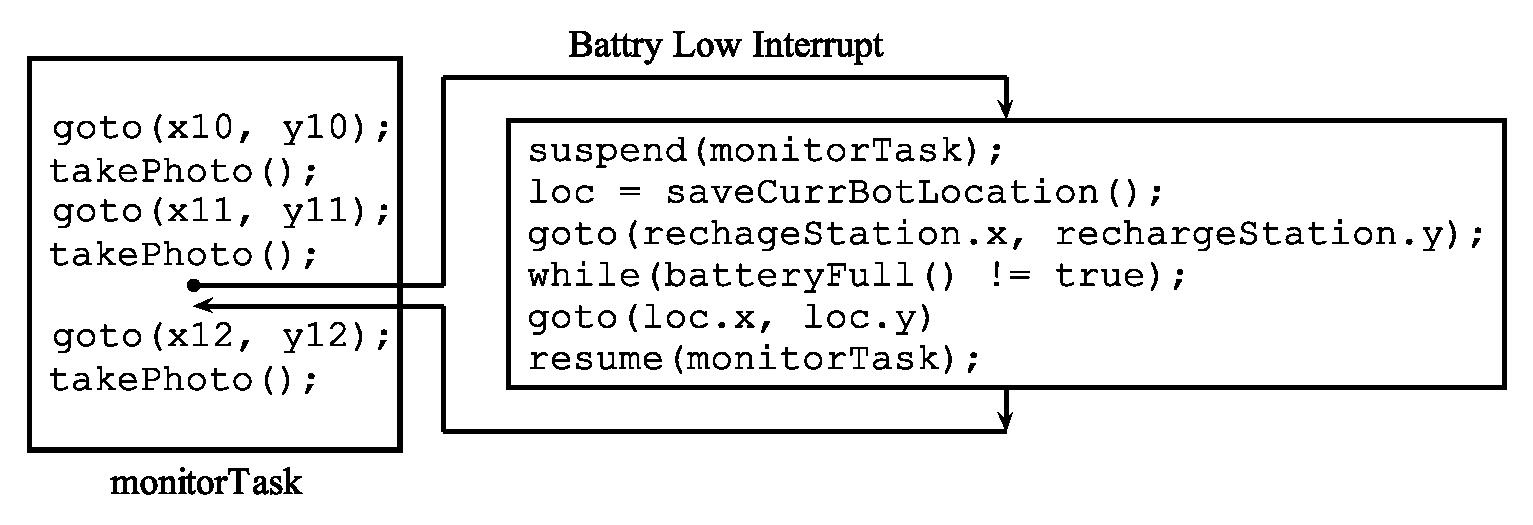
\includegraphics[scale=0.4]{./monitor}
}

\frame{\frametitle{Risk Mitigation}
 \structure{Risk \#4} Unauthorized user controls greenhouse
 
 \vspace{\baselineskip}
 Use secure network protocol and authenticate user before connection.
 }

\frame{\frametitle{Obeservations}
Problem of designing accurate and automated Bot guidance system is fundamental in nature for greenhouse applications.

\vspace{\baselineskip}
All future greenhouse projects can use this system to avoid costly or complex solutions.

\vspace{\baselineskip}
Applications who need very accurate Bot positioning just need to place \alert{extra checkpoints} at desired places.

\vspace{\baselineskip}
\hspace{0.4\textwidth} Thank You!
}

\frame{\frametitle{References}
\bibliography{sample}
}
\end{document}

